\documentclass{elektr}
\usepackage{hyperref}
\pdfinfo{
    /Author ()
    /Title ()
    /Subject ()
    /Keywords ()
}
\hypersetup{
    colorlinks=true,
    urlcolor=black,
    citecolor=blue,
    linkcolor=blue,
    pdfauthor={},
    pdftitle={},
    pdfsubject={},
    pdfkeywords={},
    pdfcreator={},
    pdfproducer={}
}
\usepackage{amsfonts,amssymb,amsmath,theorem,graphicx}
\usepackage{booktabs,array,multirow}
\usepackage[utf8]{inputenc}
\usepackage[english]{babel}
\usepackage[pagewise]{lineno}
\linenumbers
\setlength{\textfloatsep}{3.5pt plus 1pt minus 1pt}
\setlength{\intextsep}{3.5pt plus 1pt minus 1pt}
\setlength{\floatsep}{3.5pt plus 1pt minus 1pt}
\AtBeginDocument{%
  \setlength{\abovedisplayskip}{3.0pt plus 1pt minus 1pt}%
  \setlength{\belowdisplayskip}{3.0pt plus 1pt minus 1pt}%
  \setlength{\abovedisplayshortskip}{2pt plus 1pt minus 1pt}%
  \setlength{\belowdisplayshortskip}{2pt plus 1pt minus 1pt}%
}

\yil{}
\vol{}
\fpage{}
\lpage{}
\doi{}

\title{Optimal age replacement and component-mix design for heterogeneous weighted k-out-of-n:G systems under asymmetric capacity-proportional load sharing}

\author[Anonymous]{
	\textbf{Blinded for peer review}
}

\input{elksty.tex}

\setcounter{page}{1}

\begin{document}

\maketitle

\begin{abstract}Weighted k-out-of-n:G power and industrial systems pair lower-capacity Type~I and higher-capacity Type~II units to balance maintenance cost against supply adequacy. When a unit fails during a deferred-repair epoch, survivors absorb displaced load asymmetrically, and losing a larger Type~II unit triggers sharper stress escalation than losing a Type~I unit. Prior weighted-system maintenance models largely assume statistical independence or identical components. This study develops an exact Continuous-Time Markov Chain and Phase-Type framework for optimal age replacement and component-mix design under capacity-proportional Tampered Failure Rate load sharing. Closed-form matrix-exponential expressions are derived for reliability, mean time to failure, and renewal cycle costs under module replacement (Policy~I) and state-dependent component renewal (Policy~II). Using a variance--drift hazard decomposition and a two-stage solver, we establish monotone increasing hazard conditions and explain tail non-monotonicity and optimal-age reversals under severe stress. Parameterized from four IEEE Reliability Test System--Grid Modernization Lab Consortium (RTS-GMLC) arrays, GE Vernova GER-3620 Rev~P inspection factors, and U.S.\ Energy Information Administration Annual Energy Outlook 2026 cost benchmarks, the case study highlights four patterns. Inside the 1.03--1.15 overload band (90\% threshold), neglecting load sharing adds up to 3.90\% at corrective-to-preventive cost ratio 5 and 13.99\% at cost ratio 20. At a 50\% threshold, penalties reach 36.66\%--80.24\% (ratio 5) and 73.40\%--346.06\% (ratio 20) under 1.15 capping, versus 68.79\% and 277.57\% on the unthrottled lower-bound rotor branch. Across 80 configurations, 66 of 68 interior turning points lie in the 1.03--1.15 envelope (44 of 68 under 1.10--1.20), and reverse-ordered coal arrays reach corrective-only operation earlier than gas-turbine clusters. Baseline downtime pricing eliminates all 815 unpenalized inversions across 2,628 finite cases while shifting benchmark peaking ages (70\% threshold, ratio 5) by at most 3.12\%, and Policy~II mapping confirms that O\&M asymmetry drives interior mixes.

\keywords{Weighted k-out-of-n systems, load sharing, age replacement, phase-type distributions, mixed-integer nonlinear programming, power system reliability}
\end{abstract}

\section{Introduction}
\label{sec:intro}

Supply adequacy and scheduled preventive maintenance (PM) are central to electric power systems and multi-unit industrial plants. Classical adequacy evaluation uses loss-of-load probability and expected energy not supplied across capacity-rated generators \cite{rts1979,grigg1999,billinton1996,billinton1994}, modeled via Continuous-Time Markov Chains (CTMC) \cite{lisnianski2012,ding2009}. At substation, microgrid, and peaking-cluster levels, parallel generators, pumps, or chillers form weighted $k$-out-of-$n$:G structures: component $\ell \in \{1, \dots, n\}$ provides integer weight $w_\ell$, and the system operates iff total available capacity reaches demand threshold $k$ \cite{wu1994,kuo2003,rushdi2018}.

Real power stations and multi-unit cooling plants commonly mix smaller, fast-response peaking units (Type~I) with larger frame units (Type~II) to balance operating costs against reserve margins \cite{eryilmaz2014two,eryilmaz2018,qi2024}. Scheduling PM via renewal-reward age replacement balances planned renewal expenditure against unplanned failures under corrective-only maintenance (CM) \cite{barlow1965,nakagawa1985,nakagawa2005,wang2006}. However, prior weighted $k$-out-of-$n$ maintenance studies overwhelmingly assume independent unit failures \cite{hamdan2021,qi2024}. Over deferred-repair operating epochs between scheduled turnarounds, a cluster serving fixed output redistributes lost load onto survivors whenever a unit fails, accelerating degradation via Tampered Failure Rate (TFR) load sharing. Because Type~II units supply larger weights, losing a heavier unit triggers a sharper stress surge on survivors. Even with memoryless units, redundant weighted systems exhibit system-level aging, and ignoring load transfer mis-specifies replacement ages by either delaying preventive renewal under moderate stress or triggering premature renewal past severe-overload turning points.

Building on weighted-system threshold theory \cite{wu1994,eryilmaz2014two,rushdi2018}, classical age-replacement renewal models \cite{nakagawa2005}, and power-system maintenance scheduling \cite{fotuhi2014,almuhaini2017}, we formulate a two-type weighted $k$-out-of-$n$:G Markov model over deferred-repair operating epochs whose component hazards scale with lost capacity, paired with full-module and selective component renewal via exact matrix-exponential evaluation. Specifically, we provide: (i) a capacity-proportional TFR model handling both conventional peaking fleets and reverse-ordered fleets with unit-specific overload sensitivities; (ii) closed-form reliability, mean time to failure ($\mathrm{MTTF}$), and cost-rate expressions without numerical quadrature for joint mix-and-age optimization; (iii) analytical conditions explaining when PM is uniquely optimal versus when severe overload favors CM; and (iv) a parameterized case-study suite (E1--E6) for deferred-repair epochs built from four regional IEEE Reliability Test System--Grid Modernization Lab Consortium (RTS-GMLC) arrays \cite{barrows2020}, GE Vernova GER-3620 Rev~P inspection factors \cite{ger3620}, and U.S.\ Energy Information Administration (EIA) Annual Energy Outlook (AEO) 2026 operation and maintenance (O\&M) benchmarks \cite{eia2026}. Complete proofs, synthetic verification checks, and 100,000-trial Monte Carlo validations at positive overload sensitivity appear in Supplementary Sections~S1--S2.

\section{Literature review and positioning}
\label{sec:lit}

Research relevant to this study bridges weighted $k$-out-of-$n$ maintenance, dynamic load-sharing reliability, and power-system maintenance optimization.

\subsection{Weighted k-out-of-n and power-system maintenance models}
Wu and Chen \cite{wu1994} introduced weighted $k$-out-of-$n$:G state recursion, and Rushdi and Alturki \cite{rushdi2018} unified coherent threshold modeling via signal flow graphs. Extending heterogeneous systems to two types, Eryilmaz and Sarikaya \cite{eryilmaz2014two} derived survival functions, Birnbaum importances, and acquisition-cost mix rules without dynamic load redistribution or PM. Later works studied multi-state Universal Generating Functions \cite{li2008}, $\mathrm{MTTF}$ and residual capacity distributions \cite{eryilmaz2015mttf,eryilmaz2015,eryilmaz2021}, multi-type failure counts \cite{eryilmaz2018}, and survival signatures \cite{hamdan2024}. For PM, Hamdan et al.\ \cite{hamdan2021} combined weight limits with age thresholds, Qi et al.\ \cite{qi2024} scheduled inspections under independence, and Qi et al.\ \cite{qi2026} added copula correlation to condition-based maintenance (CBM). Power-system studies examined market-driven generator scheduling \cite{fotuhi2014,golmohamadi2014}, reliability-constrained commitment \cite{heidari2016}, distribution O\&M \cite{hashemi2013}, Markovian microgrids \cite{almuhaini2017}, and Petri-net protection \cite{kumari2026}, yet omit capacity-proportional TFR load redistribution.

\subsection{Load-sharing k-out-of-n reliability and maintenance}
Load sharing stems from fiber-bundle models \cite{daniels1945}, arbitrary non-i.i.d.\ load-sharing $k$-out-of-$n$ formulations \cite{liu1998}, and Markovian equal-load TFR or cumulative-exposure models \cite{amari2008,taghipour2015}. Recent studies treat degrading-component PM \cite{liu2016}, shock-induced soft/hard failures \cite{che2020,huang2023}, opportunistic PM with minimal repair \cite{jamali2022}, environmental redundancy \cite{hao2024}, and stochastic mission allocation or joint spares-and-PM inventory optimization \cite{ghnimi2025,mannai2026,zhao2025}. Weighted load-sharing PM remains scarce: Sharifi and Taghipour \cite{sharifi2023} optimized inspections under identical component weights. Rather than a formal systematic review, Table~\ref{tab:lit_positioning} synthesizes representative studies across three intersecting streams (weighted $k$-out-of-$n$ PM, load-sharing reliability and maintenance, and power-system maintenance scheduling), showing that joint component-mix and replacement-age optimization under asymmetric capacity-proportional TFR load sharing remains open.

\begin{table}[htbp]
\centering
\scriptsize
\renewcommand{\arraystretch}{0.80}
\setlength{\tabcolsep}{1.3pt}
\caption{Methodological positioning relative to reviewed reliability and power-system maintenance literature.}
\label{tab:lit_positioning}
\begin{tabular*}{\textwidth}{@{\extracolsep{\fill}}p{3.0cm}p{2.3cm}p{2.7cm}p{1.6cm}p{2.1cm}p{2.1cm}@{}}
\toprule
Study & Structure / Units & Stress / Aging & Repair & Policy & Decisions \\
\midrule
Fotuhi-Firuzabad et al.\ \cite{fotuhi2014} & Power / Heterog. & Adequacy / Const. & Scheduled & Generator PM & Outage windows \\
Almuhaini and Al-Sakkaf \cite{almuhaini2017} & Microgrid / Heterog. & Load limit / Exp. & Yes & Adequacy eval. & Reliab.\ indices \\
Eryilmaz and Sarikaya \cite{eryilmaz2014two} & Weighted $k/n$ / 2 types & Indep.\ / Exp. & No & Design (no PM) & Mix selection \\
Eryilmaz \cite{eryilmaz2018} & Std.\ $k/n$:G / Multi-type & Indep.\ / Exp. & No & Failure counts & Count dist. \\
Taghipour and Kassaei \cite{taghipour2015} & Std.\ $k/n$:G / Identical & Equal TFR / Exp. & Minimal & Inspection PM & Inspect.\ period \\
Liu \cite{liu1998} & Std.\ $k/n$:G / Non-iid & Equal LS / Arb. & No & Reliab.\ eval. & System reliab. \\
Liu et al.\ \cite{liu2016} & Load-sharing / Multi & Load share / Degr. & No & Condition / age & PM threshold \\
Hamdan et al.\ \cite{hamdan2021} & Weighted $k/n$ / Arb.\ wts. & Indep.\ / Exp. & Yes & Weight / age PM & Weight / age \\
Arabzadeh Jamali and Pham \cite{jamali2022} & Std.\ $k/n$:G / Identical & Equal TFR / Exp. & Minimal & Opport.\ PM & Prev.\ age \\
Sharifi and Taghipour \cite{sharifi2023} & Weighted $k/n$ / Identical & Symm.\ multi-state & Minimal & Inspection PM & Inspect.\ period \\
Qi et al.\ \cite{qi2024} & Weighted $k/n$ / Multi-type & Indep.\ (sig.) / Gen. & No & Inspect.\ / PM & Cycle / period \\
Hao and Zhu \cite{hao2024} & Multi-asset $k/n$ / Ident. & Equal LS + env.\ / Degr. & No & Design and PM & Redund., age \\
Zhao et al.\ \cite{zhao2025} & Std.\ $k/n$:G / Identical & Load share / Degr. & Spares & State-spec.\ PM & Size, PM, inv. \\
Qi et al.\ \cite{qi2026} & Multi-state $k/n$ / Multi & Static copula / Degr. & Yes & CBM policy & Cond.\ triggers \\
Mannai and Jarray \cite{mannai2026} & Std.\ $k/n$:G / Identical & Cumul.\ exp.\ / Weibull & No & Mission design & Redund.\ alloc. \\
\textbf{This study} & \textbf{Weighted $k/n$ / 2 types} & \textbf{Asymm.\ TFR / Exp.} & \textbf{Deferred (No)} & \textbf{Module / comp.\ PM} & \textbf{Joint mix \& age} \\
\bottomrule
\end{tabular*}
\end{table}

\section{Mathematical methodology}
\label{sec:math}

\subsection{Heterogeneous weighted system and independent baseline}
Consider a parallel system of $n$ components partitioned into $m \in \{0, \dots, n\}$ Type~I units (weight $w_1 \in \mathbb{Z}^+$, baseline failure rate $\lambda_{1,0} > 0$) and $n - m$ Type~II units (weight $w_2 \in \mathbb{Z}^+$ with $w_2 > w_1$, baseline rate $\lambda_{2,0} > 0$). Unlike restrictive homogeneity assumptions, baseline ordering is left unrestricted ($\lambda_{1,0} \neq \lambda_{2,0}$), spanning both gas-turbine fleets ($\lambda_{1,0} > \lambda_{2,0}$) and reverse-order coal arrays ($\lambda_{2,0} > \lambda_{1,0}$). Let $N_1(t) \in \{0, \dots, m\}$ and $N_2(t) \in \{0, \dots, n-m\}$ denote surviving component counts at time $t \ge 0$. Active system capacity in state $(i, j)$ is $W_{i,j} = i w_1 + j w_2$, with initial capacity $W_0 = m w_1 + (n - m) w_2$. Requiring $W_{i,j} \ge k$ ($\min(w_1, w_2) \le k \le W_0$) partitions the state space $\mathcal{S}$ into working and failed sets:
\begin{equation}
\mathcal{W} = \{(i, j) \in \mathcal{S} : i w_1 + j w_2 \ge k\}, \qquad \mathcal{F} = \{(i, j) \in \mathcal{S} : i w_1 + j w_2 < k\},
\label{eq:state_partition}
\end{equation}
with $M = |\mathcal{W}|$. Under statistical independence \cite{wu1994,nakagawa2005,eryilmaz2014two}, lifetimes remain exponential with constant rates $\lambda_{1,0}, \lambda_{2,0}$, yielding the double-binomial independent-baseline ($ind$) reliability:
\begin{equation}
R_{sys}^{ind}(t) = \sum_{i=0}^{m} \sum_{j=0}^{n-m} \mathbb{I}(i w_1 + j w_2 \ge k) \binom{m}{i} \left(e^{-\lambda_{1,0} t}\right)^i \left(1 - e^{-\lambda_{1,0} t}\right)^{m - i} \binom{n - m}{j} \left(e^{-\lambda_{2,0} t}\right)^j \left(1 - e^{-\lambda_{2,0} t}\right)^{n - m - j}.
\label{eq:R_ind}
\end{equation}

\subsection{Capacity-proportional TFR load sharing and CTMC formulation}
Under active load sharing, surviving units absorb displaced load whenever failures shrink active capacity below $W_0$. Modeling an unthrottled constant-output epoch carrying initial load $W_0$, any surviving state $(i, j) \in \mathcal{W}$ subjects active units to overload ratio $\rho_{i,j} = W_0 / W_{i,j} \ge 1$ (excluding part-load operation below $W_0$). Under nameplate-capped demand-tracking dispatch ($\rho_{i,j}^{\mathrm{cap}} = \min(\rho_{\max}, W_0/W_{i,j})$ at $\rho_{\max} = 1.15$, evaluated explicitly in Section~\ref{sec:e1_e2}), overloads stay bounded within peak capability; here $k/W_0 = 0.90$ captures peak-reserve operation inside $[1.03, 1.15]$, whereas lower $k/W_0$ without capping serves as an unconstrained deep-cascade stress test. Under TFR scaling with exponents $\gamma_r \ge 0$ for Type~$r \in \{1, 2\}$ ($\gamma_1, \gamma_2$), the surviving Type~$r$ failure rate is:
\begin{equation}
\lambda_1(i, j) = \lambda_{1,0} \left( \frac{W_0}{i w_1 + j w_2} \right)^{\gamma_1}, \qquad \lambda_2(i, j) = \lambda_{2,0} \left( \frac{W_0}{i w_1 + j w_2} \right)^{\gamma_2}.
\label{eq:lam12}
\end{equation}
Setting $\gamma_1 = \gamma_2 = 0$ recovers (\ref{eq:R_ind}). Because $w_2 > w_1$, losing a Type~II unit ($W_{i,j-1} = W_{i,j} - w_2$) induces a sharper hazard surge than losing a Type~I unit. Lacking outage-load logs, $\gamma_r$ ($r \in \{1, 2\}$) maps overload ratio $\rho$ to original equipment manufacturer (OEM) factored-hours inspection multipliers ($\mathrm{MF}(\rho)$, used here as an accelerating-stress proxy rather than a direct hazard ratio) between effective rate $\lambda_{r,\mathrm{eff}}(\rho)$ and $\lambda_{r,0}$ (Section~\ref{sec:case_data}):
\begin{equation}
\text{\textbf{Accelerating-Stress Proxy Hypothesis:}} \qquad \frac{\lambda_{r,\mathrm{eff}}(\rho)}{\lambda_{r,0}} = \mathrm{MF}(\rho) \implies \gamma_r(\rho) = \frac{\ln(\mathrm{MF})}{\ln(\rho)}, \qquad \rho > 1.
\label{eq:proxy_hyp}
\end{equation}

We model non-repairable deferred-repair operating epochs between scheduled turnarounds \cite{nakagawa2005,amari2008,taghipour2015,mannai2026}, setting online repair rates to zero ($\mu_r = 0$). Fast online restoration with unit mean time to repair $\mathrm{MTTR}_r$ ($\mu_r = 1/\mathrm{MTTR}_r \gg \lambda_{r,0}$) breaks acyclicity and flattens the system hazard toward $t^* \to \infty$, an effect quantified via a repairable-CTMC extension in Section~\ref{sec:e1_e2}. Under deferred repair, $\{(N_1(t), N_2(t)), t \ge 0\}$ forms an acyclic CTMC over $\mathcal{W}$, with $\mathcal{F}$ lumped into a single absorbing state $\mathcal{F}_{abs}$. Descending lexicographic ordering from $(m, n - m)$ yields an upper-triangular $M \times M$ generator $\mathbf{Q}_{\mathcal{W}}$ with transitions $q_{(i,j)\to(i-1,j)} = i\lambda_1(i, j)$ when $(i-1, j) \in \mathcal{W}$, $q_{(i,j)\to(i,j-1)} = j\lambda_2(i, j)$ when $(i, j-1) \in \mathcal{W}$, exit rate $\nu_{i,j} = i\lambda_1(i, j) + j\lambda_2(i, j) > 0$, and diagonal $-\nu_{i,j}$.

Let $\mathbf{e} = [1, \dots, 1]^{\top}$ be the $M$-vector of ones, $\mathbf{I}_M$ the $M \times M$ identity matrix, and $T_{sys} = \inf\{t \ge 0 : (N_1(t), N_2(t)) \in \mathcal{F}\}$ the system lifetime. Direct fatal absorption rates form vector $\mathbf{q}_F = -\mathbf{Q}_{\mathcal{W}}\mathbf{e}$ with components $q_{F,(i,j)} = q_{(i,j)\to\mathcal{F}}^{(1)} + q_{(i,j)\to\mathcal{F}}^{(2)}$, where $q_{(i,j)\to\mathcal{F}}^{(1)} = i\lambda_1(i, j)\mathbb{I}((i-1, j) \in \mathcal{F})$ and $q_{(i,j)\to\mathcal{F}}^{(2)} = j\lambda_2(i, j)\mathbb{I}((i, j-1) \in \mathcal{F})$. Starting from $\boldsymbol{\alpha} = [1, 0, \dots, 0]$, the transient state probability vector $\mathbf{P}_{\mathcal{W}}(t) = [P_{i,j}(t)]$ satisfies $\mathbf{P}_{\mathcal{W}}'(t) = \mathbf{P}_{\mathcal{W}}(t)\mathbf{Q}_{\mathcal{W}}$, yielding exact matrix-exponential Phase-Type (PH) expressions for $R_{sys}(t)$, failure density $f_{sys}(t)$, expected renewal cycle duration $E[S(t)] = E[\min(T_{sys}, t)]$, and $\mathrm{MTTF}$:
\begin{align}
R_{sys}(t) &= \boldsymbol{\alpha} \exp(\mathbf{Q}_{\mathcal{W}} t) \mathbf{e}, \qquad f_{sys}(t) = \boldsymbol{\alpha} \exp(\mathbf{Q}_{\mathcal{W}} t) \mathbf{q}_F, \label{eq:R_f} \\
E[S(t)] &= \boldsymbol{\alpha} \mathbf{Q}_{\mathcal{W}}^{-1} \left( \exp(\mathbf{Q}_{\mathcal{W}} t) - \mathbf{I}_M \right) \mathbf{e}, \qquad \mathrm{MTTF} = -\boldsymbol{\alpha} \mathbf{Q}_{\mathcal{W}}^{-1} \mathbf{e}, \label{eq:ES_MTTF}
\end{align}
where nonsingularity of upper-triangular $\mathbf{Q}_{\mathcal{W}}$ avoids numerical quadrature entirely.

\subsection{Maintenance policies and expected cost rates}
Under age replacement, the system is renewed preventively at operational age $t > 0$ or correctively upon failure ($T_{sys} < t$), whichever occurs first. Sections~3--5.4 assume instantaneous renewals (preventive and corrective outage durations $d_{PM} = d_{CM} = 0$), while Section~\ref{sec:e6} relaxes this via reported unit restoration durations.

\paragraph{Policy~I (Complete module replacement):} Replacing the full module at operational age $t > 0$ costs $c_1$, while CM failure replacement costs $c_2 > c_1$. Denoting the renewal-reward long-run expected cost per unit time (cost rate) by $\eta(t)$, (\ref{eq:R_f})--(\ref{eq:ES_MTTF}) give Policy~I cost rate $\eta_I(t)$:
\begin{equation}
\eta_I(t) = \frac{c_2 - (c_2 - c_1) R_{sys}(t)}{\int_{0}^{t} R_{sys}(u)\,du} = \frac{c_2 - (c_2 - c_1) \boldsymbol{\alpha} \exp(\mathbf{Q}_{\mathcal{W}} t) \mathbf{e}}{\boldsymbol{\alpha} \mathbf{Q}_{\mathcal{W}}^{-1} \left( \exp(\mathbf{Q}_{\mathcal{W}} t) - \mathbf{I}_M \right) \mathbf{e}}.
\label{eq:etaI}
\end{equation}

\paragraph{Policy~II (State-dependent component renewal):} For modular multi-unit systems maintained at scheduled turnarounds, discarding unfailed Type~II units is avoidable. Upon any intervention in $(i, j) \in \mathcal{W}$ (at age $t$) or $(i', j') \in \mathcal{F}$ (upon failure), failed units are replaced at unit costs $c_{rep,1}, c_{rep,2}$, while surviving units receive minor preventive servicing ($c_{ref,1} \ll c_{rep,1}$, $c_{ref,2} \ll c_{rep,2}$), alongside setup cost $c_0$ and CM outage penalty $c_{pen}$:
\begin{align}
C_{PM}(i, j) &= c_0 + (m - i) c_{rep,1} + (n - m - j) c_{rep,2} + i c_{ref,1} + j c_{ref,2}, \label{eq:CPM} \\
C_{CM}(i', j') &= c_0 + c_{pen} + (m - i') c_{rep,1} + (n - m - j') c_{rep,2} + i' c_{ref,1} + j' c_{ref,2}. \label{eq:CCM}
\end{align}
Because baseline lifetimes are memoryless and TFR rates depend only on current counts $(i, j)$, replacing failed units and servicing survivors regenerates state $(m, n-m)$ as good as new. Defining absorption cost rates $c_{abs,(i,j)} = q_{(i,j)\to\mathcal{F}}^{(1)} C_{CM}(i-1, j) + q_{(i,j)\to\mathcal{F}}^{(2)} C_{CM}(i, j-1)$ yields the closed-form cost rate:
\begin{equation}
\eta_{II}(m, t) = \frac{\sum_{(i,j) \in \mathcal{W}} P_{i,j}(t) C_{PM}(i, j) + \boldsymbol{\alpha}\mathbf{Q}_{\mathcal{W}}^{-1}\left(\exp(\mathbf{Q}_{\mathcal{W}} t) - \mathbf{I}_M\right)\mathbf{c}_{abs}}{\boldsymbol{\alpha} \mathbf{Q}_{\mathcal{W}}^{-1} \left( \exp(\mathbf{Q}_{\mathcal{W}} t) - \mathbf{I}_M \right) \mathbf{e}}.
\label{eq:etaII}
\end{equation}

\subsection{Analytical properties and global-to-local optimization solver}
Complete proofs appear in Supplementary Section~S1. First, by monotonicity of $(W_0/W_{i,j})^{\gamma_r}$ for $\gamma_r > 0$, surviving unit hazards rise strictly after any non-fatal failure, with a strictly larger jump after Type~II loss whenever both $(i-1,j)$ and $(i,j-1)$ remain operational ($\lambda_r(i, j-1) > \lambda_r(i-1, j) > \lambda_r(i, j)$, \textbf{Lemma~1}). Second, differentiating the conditional state vector $\mathbf{p}(t) = \mathbf{P}_{\mathcal{W}}(t)/R_{sys}(t)$ yields the exact hazard-rate decomposition:
\begin{proposition}[Variance--Drift Decomposition]
Let $h_{sys}(t) = f_{sys}(t)/R_{sys}(t) = \mathbf{p}(t)\mathbf{q}_F$ be the system hazard rate given $T_{sys} > t$. For $M \ge 2$,
\begin{equation}
\frac{d h_{sys}(t)}{dt} = -\operatorname{Var}_{\mathbf{p}(t)}(\mathbf{q}_F) + \sum_{x \in \mathcal{W}} p_x(t) \sum_{y \neq x, \, y \in \mathcal{W}} Q_{xy} \left(q_{F,y} - q_{F,x}\right).
\label{eq:dh_decomp}
\end{equation}
Eq.~(\ref{eq:dh_decomp}) decomposes $dh_{sys}(t)/dt$ into survivor-selection variance and transition drift, yielding positive slope at $t$ precisely when drift exceeds variance. Thus, for any unbranched operational chain with $M_{\mathrm{eff}} \ge 2$ effective phases ($M_{\mathrm{eff}} = M$ when $m=0$ or $m=n$, or $M_{\mathrm{eff}} = n - \lceil k/w_1 \rceil + 1$ in the homogeneous symmetric limit $w_1=w_2, \lambda_{1,0}=\lambda_{2,0}, \gamma_1=\gamma_2$), the decomposition and phase convolution unconditionally establish strict Increasing Failure Rate (IFR) behavior ($dh_{sys}(t)/dt > 0$ for all $t > 0$).
\end{proposition}
Eq.~(\ref{eq:dh_decomp}) explains why branching two-type PH distributions are \emph{not} unconditionally IFR (\textbf{Remark~1}): in the dimensionless 15-unit synthetic benchmark ($w_1=1, w_2=2, k=15$; Supplementary Section~S2), once fast-absorbing Type~I paths saturate, late-time survival conditions onto slower Type~II paths and can yield $dh_{sys}(t)/dt < 0$ over localized tail intervals for $m \in \{5,6,8\}$ ($t \in [17.6, 22.4]$, $[14.6, 33.0]$, $[9.7, 14.2]$) or across the asymptotic tail $t \ge 14.0$ for $m = 7$ (truncated at $t = 36.7$ by the $10^{-15}$ survival-precision floor in Supplementary Figure~S1c, all at $R_{sys}(t) \le 2.80 \times 10^{-4}$).

Third, differentiating $\eta_I(t)$ yields $d \eta_I(t)/dt \propto g(t) = h_{sys}(t)\int_0^t R_{sys}(u)\,du - [1 - R_{sys}(t)] - \frac{c_1}{c_2-c_1}$ (\textbf{Theorem~1}, specializing the classical renewal-reward optimality criterion \cite{barlow1965,nakagawa2005} to PH expressions (\ref{eq:R_f})--(\ref{eq:ES_MTTF})). Under IFR and $\lim_{t\to\infty} h_{sys}(t)\,\mathrm{MTTF} > c_2/(c_2-c_1)$, $t^* \in (0, \infty)$ is the unique finite global minimum; otherwise $t^* \to \infty$ (CM), and in branching cases global optimality is resolved numerically via Algorithm~S1.

Finally, two boundary limits govern extreme load sharing (\textbf{Theorem~2}). As $\gamma_1, \gamma_2 \to 0$, $R_{sys} \to R_{sys}^{ind}$ uniformly on compact intervals and $t^* \to t_{ind}^*$ whenever $t_{ind}^*$ is the unique minimizer on search bracket $[t_{lb}, t_{ub}]$ (or both enter CM). As $\gamma_1, \gamma_2 \to \infty$, degraded-state hazards explode and collapse reliability to the memoryless first-failure limit $\exp(-(m\lambda_{1,0}+(n-m)\lambda_{2,0})t)$, forcing $t^* \to \infty$. While these two limits do not prove unimodality analytically, numerical sweeps consistently show $t^*(\gamma)$ decreasing initially at low $\gamma$, attaining a minimum at turning point $\gamma_{\mathrm{tp}}$, and then bending upward toward $\infty$ (\textbf{Remark~2}).

Joint mix-and-age optimization solves the mixed-integer nonlinear program (MINLP):
\begin{equation}
\min_{m \in \{0, 1, \dots, n\}, \, t > 0} \eta(m, t) \quad \text{subject to} \quad m w_1 + (n - m) w_2 \ge k.
\label{eq:minlp}
\end{equation}
Because bounded Brent probes drift in flat $R_{sys}(t) \approx 0$ tails, a two-stage solver (Supplementary Algorithm~S1) screens a 300-point two-segment grid over $[t_{lb}, \max(t_{ub}, 6\,\mathrm{MTTF})]$ (extending to $20\,\mathrm{MTTF}$ if needed), tests $\eta(\infty)$ within $10^{-12}$, and refines via Brent search (tolerance $10^{-9}$; $t_{lb} = \max(0.5, 10^{-3}\,\mathrm{MTTF}), t_{ub} \le 2000\;\text{h}$ for RTS-GMLC).

\section{Case-study parameterization from IEEE RTS-GMLC arrays}
\label{sec:case_data}

This section parameterizes the deferred-repair case study ($\mu_r = 0$) from regional power-system arrays, OEM stress curves, and utility O\&M benchmarks. Exact $\gamma = 0$ benchmark checks and 100,000-trial Monte Carlo validations of the PH matrix-exponential evaluator at positive $\gamma$ appear in Supplementary Section~S2; online repair (Section~\ref{sec:e1_e2}) and non-zero restoration durations (Section~\ref{sec:e6}) are evaluated directly in the results.

\subsection{Area-based RTS-GMLC arrays and reliability mapping}
Grouping all 158 RTS-GMLC generators \cite{barrows2020} strictly by zone (Zones~100, 200, and~300) yields three combustion-turbine (CT) peaking clusters combining \texttt{U20} oil CTs ($w_1 = 20\;\text{MW}$) and \texttt{U55} gas CTs ($w_2 = 55\;\text{MW}$), plus a reverse-order coal cluster (\texttt{U76} + \texttt{U155}) in Area~1 ($\lambda_{2,0} > \lambda_{1,0}$). All 105,408 five-minute regional load intervals confirm an identical $2{,}850.0\;\text{MW}$ peak per area; each $465$--$685\;\text{MW}$ CT cluster serves $16\%$--$24\%$ of area peak demand, motivating $k/W_0 \in \{0.50, 0.60, 0.70, 0.80, 0.90\}$ with $k = \lceil (k/W_0) W_0 \rceil$ and reported $\mathrm{MTTF}$, mean time to repair ($\mathrm{MTTR}$), and forced outage rate ($\mathrm{FOR}$) (Table~\ref{tab:rts_arrays}).

\begin{table}[htbp]
\centering
\scriptsize
\renewcommand{\arraystretch}{0.80}
\setlength{\tabcolsep}{2.5pt}
\caption{IEEE RTS-GMLC regional generating arrays \cite{barrows2020}.}
\label{tab:rts_arrays}
\begin{tabular*}{\textwidth}{@{\extracolsep{\fill}}lccccccccc@{}}
\toprule
Array & Composition & $n$ & As-built $m$ & $W_0$ (MW) & $w_1, w_2$ & $\mathrm{MTTF}_{1,2}$ (h) & $\mathrm{MTTR}_{1,2}$ (h) & $\mathrm{FOR}_{1,2}$ & Ordering \\
\midrule
CT Area 1   & $4\times\texttt{U20} + 7\times\texttt{U55}$  & 11 & 4 & 465 & 20, 55  & 450, 969  & 50, 31 & 0.100, 0.031 & $\lambda_1 > \lambda_2$ \\
CT Area 2   & $4\times\texttt{U20} + 9\times\texttt{U55}$  & 13 & 4 & 575 & 20, 55  & 450, 969  & 50, 31 & 0.100, 0.031 & $\lambda_1 > \lambda_2$ \\
CT Area 3   & $4\times\texttt{U20} + 11\times\texttt{U55}$ & 15 & 4 & 685 & 20, 55  & 450, 969  & 50, 31 & 0.100, 0.031 & $\lambda_1 > \lambda_2$ \\
Coal Area 1 & $4\times\texttt{U76} + 3\times\texttt{U155}$ & 7  & 4 & 769 & 76, 155 & 1960, 960 & 40, 40 & 0.020, 0.040 & $\lambda_2 > \lambda_1$ \\
\bottomrule
\end{tabular*}
\end{table}

Without weight scaling, weights equal MW ratings ($w_r$) with baseline rates $\lambda_{r,0} = 1/\mathrm{MTTF}_r$: $2.222 \times 10^{-3}\;\text{h}^{-1}$ (\texttt{U20}), $1.032 \times 10^{-3}\;\text{h}^{-1}$ (\texttt{U55}), $5.102 \times 10^{-4}\;\text{h}^{-1}$ (\texttt{U76}), and $1.042 \times 10^{-3}\;\text{h}^{-1}$ (\texttt{U155}), where $\mathrm{FOR} = \mathrm{MTTR}/(\mathrm{MTTF} + \mathrm{MTTR})$ holds to $< 10^{-6}$. Interpreting RTS-GMLC $\mathrm{MTTF}$ entries as active-commitment service hours defines a fired-hour modeling premise for our peaking study; $t^*$ converts to calendar years via capacity factor $\mathrm{CF}$ as $t_{\mathrm{cal}} = t_{\mathrm{fired}}/(\mathrm{CF}\cdot 8760)$ ($100$--$300\;\text{h}$ spans $0.07$--$3.42\;\text{yr}$ at $1\%$--$17\%$ duty \cite{ger3620}).

\subsection{Stress-exponent calibration via OEM mechanism curves}
Invoking (\ref{eq:proxy_hyp}) from Section~3.2, we evaluate dimensionless maintenance factors ($\mathrm{MF}$) from GE Vernova GER-3620 Rev~P \cite{ger3620}, which parameterizes peak duty via a $+100^{\circ}\text{F}$ firing-temperature adder without stating a generic MW or percentage electrical output increment $\rho = P_{\mathrm{peak}}/P_{\mathrm{base}}$ (peak-to-base power output ratio). Accordingly, $\gamma(\rho)$ is calibrated over $\rho \in [1.03, 1.15]$ along two physical curves (Figure~\ref{fig:mechanism_curves}a). The lower-bound \textbf{Rotor branch} ($\mathrm{MF} = 2.00$, Figure~44, p.~35 of \cite{ger3620}) comes from $\mathrm{MF} = (H_{\mathrm{base}} + 2 H_{\mathrm{peak}})/(H_{\mathrm{base}} + H_{\mathrm{peak}})$ at $100\%$ peak duty ($H_{\mathrm{base}} = 0$; called $H, P$ in \cite{ger3620}, renamed to avoid collision with $P_{i,j}, P_{\mathrm{peak}}$), spanning $\gamma \in [4.96, 23.45]$ ($4.96, 6.12, 7.27, 9.01, 14.21, 23.45$ at $\rho = 1.15, 1.12, 1.10, 1.08, 1.05, 1.03$). The upper-bound \textbf{hot-gas-path (HGP) heavy-duty B- and E-class (B/E-class) branch} ($\mathrm{MF} = 6.05$, Figure~10 and Appendix~A.1, pp.~7, 39 of \cite{ger3620}) uses the peak load-severity factor $A_p = \exp(0.018\, T_f)$ at firing-temperature adder $T_f = +100^{\circ}\text{F}$ ($e^{1.8} \approx 6.0496$, rounded to $\mathrm{MF} = 6.05$), spanning $\gamma \in [12.88, 60.90]$ ($12.88, 15.88, 18.89, 23.39, 36.89, 60.90$; F-class $e^{2.3} \approx 9.9742$ yields $\gamma \in [16.46, 77.81]$ as reference).

Only tight demand thresholds ($k/W_0 = 0.90$, $\max W_0/W_{i,j} = 1.110$) stay inside $\rho \in [1.03, 1.15]$; lower thresholds such as $k/W_0 = 0.50$ reach attained state ratios $\max_{(i,j)\in\mathcal{W}} W_0/W_{i,j} \in [1.938, 1.957]$ across CT Areas~1--3 and $1.992$ in Coal Area~1 (bounded by the discrete ceiling $W_0/\lceil 0.50\,W_0\rceil = 1.996$--$1.997$, below the continuous limit $2.000$), treating (\ref{eq:lam12}) as an unconstrained deep-cascade extrapolation. Below base load, \cite{ger3620} assigns $\mathrm{MF} = 0.5$ on starts criteria ($<60\%$ load) and $A_p = 1.0$ on hours-based HGP criteria, confirming our part-load exclusion.

\subsection{Dimensionless O\&M cost-ratio derivation}
Following EIA AEO 2026 (Table~3, 2025 dollars) \cite{eia2026}, greenfield capital costs are excluded because age replacement optimizes ongoing operations. Matching aeroderivative CT fixed and variable O\&M ($\mathrm{FOM}_1 = \$9.99/\text{kW-yr}$, $\mathrm{VOM}_1 = \$5.97/\text{MWh}$) to \texttt{U20} and industrial-frame CT O\&M ($\mathrm{FOM}_2 = \$7.18/\text{kW-yr}$, $\mathrm{VOM}_2 = \$4.17/\text{MWh}$) to \texttt{U55} at $\mathrm{CF} = 0.10$ ($876\;\text{h/yr}$) gives $\$304.4\text{k/yr}$ per \texttt{U20} versus $\$595.8\text{k/yr}$ per \texttt{U55}, fixing the Policy~II unit O\&M ratio for CT arrays:
\begin{equation}
r_{\mathrm{OM}} = \frac{c_{rep,2}}{c_{rep,1}} = \frac{c_{ref,2}}{c_{ref,1}} = \frac{55 \times (7.18 + 4.17 \times 0.876)}{20 \times (9.99 + 5.97 \times 0.876)} = 1.9574 \approx 1.96,
\label{eq:eia_unit_ratio}
\end{equation}
which varies only over $1.950$--$1.976$ across $\mathrm{CF} \in [0\%, 17\%]$, assuming event renewals scale with annual component O\&M. For Policy~I (theoretical single-cluster bound), emergency mobilization ($\kappa_{\mathrm{emerg}} \in [1.5, 2.5]$) plus $31$--$50\;\text{h}$ shortfall risk (illustrated by $100$--$300\;\text{MW}$ at $\$500$--$\$2{,}000/\text{MWh}$) relative to Area~1 O\&M ($4 \times \$304.4\text{k} + 7 \times \$595.8\text{k} = \$5.39\text{M/yr}$) motivates $c_2/c_1 \in \{3, 5, 10, 20\}$ ($c_1 = 1$). For Policy~II (E4), we normalize Type~I replacement to $c_{rep,1} = 1.0$ and use uncalibrated illustrative baseline ratios for minor preventive servicing ($c_{ref,1} = 0.15$) and fixed setup ($c_0 = 2.0$), scaling Type~II rates via $c_{rep,2} = r_{\mathrm{OM}} c_{rep,1}$ and $c_{ref,2} = r_{\mathrm{OM}} c_{ref,1}$ (sensitivity to $c_0$ and $c_{ref,1}$ is tested in Section~\ref{sec:e4}). These baselines span a 4D box over $r_{\mathrm{OM}} \in \{1.00, 1.50, 1.9574, 2.50, 3.00\}$, $c_{pen} \in \{10, 15, 25, 40, 100\}$, $k/W_0 \in \{0.50, 0.60, 0.70, 0.80, 0.90\}$, and the 10-point $\gamma$ grid $\{0.00, 4.96, 7.27, 9.01, 12.88, 14.21, 18.89, 23.45, 36.89, 60.90\}$. Defining the intact-state preventive cost $C_{PM,\mathrm{ref}} = C_{PM}(m, n-m)$, this box spans effective corrective-to-preventive ratios $c_2/c_{1,\mathrm{eff}} = (C_{PM,\mathrm{ref}} + c_{pen})/C_{PM,\mathrm{ref}} \in [2.32, 28.40]$ at $m = 4$ with fixed demand $k = \lceil (k/W_0) W_{0,\mathrm{as\text{-}built}} \rceil$.

\section{Results and discussion}
\label{sec:results}

Experiments~E1--E6 cover the $\gamma = 0$ baseline (E1), OEM symmetric/asymmetric curves (E2), turning-point sweeps (E3), 4D Policy~II mix maps (E4), Coal counterfactuals (E5), and MTTR downtime sensitivity (E6).

\subsection{E1 and E2: independent baseline versus symmetric and asymmetric OEM curves}
\label{sec:e1_e2}

Figures~\ref{fig:mechanism_curves}b--c trace optimal age $t^*$ and the naive load-sharing ($LS$) versus independent ($ind$) penalty $\Delta\eta\% = [\eta_{LS}(t_{ind}^*) - \eta_{LS}^*]/\eta_{LS}^* \times 100\%$ along both OEM curves at $k/W_0 = 0.70, c_2/c_1 = 5$, while Table~\ref{tab:case_e1_e2} and Supplementary Table~S5 summarize disjoint subsets of the 480-case E2 grid ($\rho \in \{1.15, 1.10, 1.05, 1.03\}$). Inside the calibrated overload band ($k/W_0 = 0.90$, attained $\max W_0/W_{i,j} = 1.094$, $1.106$, and $1.096$ in CT Areas~1--3 and $1.110$ in Coal Area~1), CT Area~1 ($k = 419\;\text{MW}$, margin $46\;\text{MW} < w_2$) fails upon losing any \texttt{U55} ($M = 3$). Consequently, penalties at $c_2/c_1 = 5$ remain $\le 1.41\%$ at $\rho = 1.15$ and $\le 3.90\%$ across $\rho \in [1.03, 1.15]$ (CT Area~2, HGP $\rho = 1.03$), rising to $+13.99\%$ at $c_2/c_1 = 20$ (CT Area~1, Rotor $\rho = 1.03$). At $k/W_0 = 0.50$, imposing nameplate-capped dispatch ($\rho_{i,j}^{\mathrm{cap}} = \min(1.15, W_0/W_{i,j})$ in CT Area~3) still produces $\mathrm{MTTF} = 369.61\;\text{h}$ and a $36.66\%$ penalty ($t^* = 192.14\;\text{h}$) at Rotor $\gamma = 4.96, c_2/c_1 = 5$ ($73.40\%$ at $c_2/c_1 = 20$), and an $80.24\%$ penalty ($t^* = 85.18\;\text{h}$, $\mathrm{MTTF} = 172.28\;\text{h}$) at HGP $\gamma = 12.88$ ($346.06\%$ at $c_2/c_1 = 20$).

Under unthrottled deep-cascade extrapolation ($k/W_0 = 0.50$), Rotor penalties at $c_2/c_1 = 5$ climb to $+44.10\%$ (Area~1), $+56.88\%$ (Area~2), and $+68.79\%$ (Area~3), whereas HGP compresses to $+25.05\%$ because severe cascaded hazards push the cluster past its turning point toward flat weakest-link CM behavior. At $c_2/c_1 = 20, \rho = 1.15$ in Area~3, unthrottled penalties peak at $+277.57\%$ (Rotor) and $+170.93\%$ (HGP). Across $\rho \in [1.03, 1.15]$ at $c_2/c_1 = 5$, Rotor retains finite PM almost everywhere ($26.10\%$--$43.11\%$ below CM for $k/W_0 \in [0.50, 0.70]$ at $\rho = 1.15$; Tables~\ref{tab:case_e1_e2} and~S5), whereas HGP B/E reaches $t^* = \infty$ for $\rho \le 1.05$ ($\gamma \ge 36.89$).

To test the deferred-repair boundary, we extend the CTMC on $\mathcal{W}$ with independent parallel online unit repair transitions $(i, j) \to (i+1, j)$ at rate $(m - i)\mu_1$ and $(i, j) \to (i, j+1)$ at rate $(n - m - j)\mu_2$ (with $\mathcal{F}$ remaining absorbing), setting $\mu_1 = 1/50\;\text{h}^{-1}$ and $\mu_2 = 1/31\;\text{h}^{-1}$. On CT Area~1 ($k/W_0 = 0.70, \gamma = 4.96, c_2/c_1 = 5$), online repair lifts $\mathrm{MTTF}$ from $182.89$ to $942.63\;\text{h}$ and flattens the asymptotic quasi-stationary hazard rate $h_\infty = \lim_{t\to\infty} h_{sys}(t)$ to $1.1157\times 10^{-3}\;\text{h}^{-1}$ ($h_\infty \mathrm{MTTF} = 1.0517 < 1.25$), collapsing the optimal policy to corrective-only replacement ($t^* = \infty$).

To test heterogeneous stress ($\gamma_1 \neq \gamma_2$), E2b evaluates all four $(\mathrm{Rotor}, \mathrm{HGP})$ pairs across CT Areas~1--3 and $\rho \in \{1.15, 1.10, 1.03\}$ (720 evaluations; 12 rows at $k/W_0 = 0.70, c_2/c_1 = 5, \rho = 1.15$ in Supplementary Table~S8). In as-built CT Areas~1--3 ($m=4, n-m \in \{7,9,11\}$), elevating Type~II (\texttt{U55}) stress cuts Area~1 $\mathrm{MTTF}$ from $182.89$ to $117.49\;\text{h}$ ($t^*$ from $88.58$ to $63.62\;\text{h}$, near all-HGP $108.25$ and $64.46\;\text{h}$) versus $155.43\;\text{h}$ ($80.75\;\text{h}$) for Type~I (\texttt{U20}) alone, matching Areas~2 ($148.14$ versus $111.17\;\text{h}$) and~3 ($154.83$ versus $106.42\;\text{h}$). Because $n-m > m$ confounds unit weight ($55 > 20\;\text{MW}$) with unit count, an equal-count control ($5\times\texttt{U20} + 5\times\texttt{U55}$, $W_0 = 375\;\text{MW}, k = 263\;\text{MW}$) isolates weight asymmetry cleanly ($\mathrm{MTTF} = 117.83\;\text{h}, t^* = 67.51\;\text{h}$ for $\gamma_2 = 12.88$ versus $130.63\;\text{h}, 96.31\;\text{h}$ for $\gamma_1 = 12.88$).

\begin{figure}[htbp]
\centering
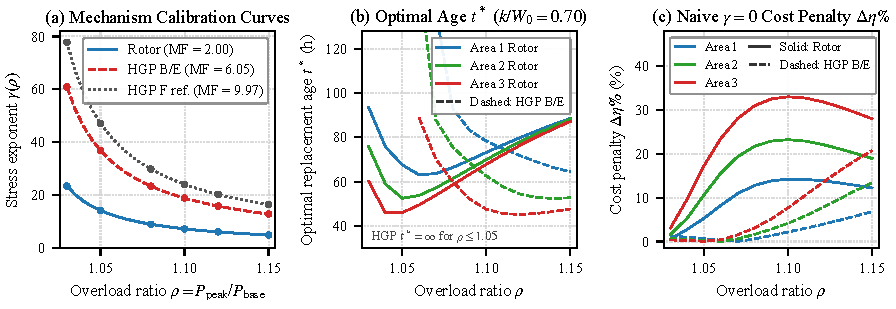
\includegraphics[width=14.5cm]{../figures/fig1_mechanism_curves.pdf}
\caption{OEM calibration and E2 response ($\rho = P_{\mathrm{peak}}/P_{\mathrm{base}}$): (a) $\gamma(\rho)$ along Rotor ($\mathrm{MF} = 2.00$), HGP B/E ($\mathrm{MF} = 6.05$), and HGP F ($\mathrm{MF} = 9.97$); (b) optimal age $t^*$ and (c) naive penalty $\Delta\eta\%$ across CT Areas~1--3 ($k/W_0 = 0.70, c_2/c_1 = 5$).}
\label{fig:mechanism_curves}
\end{figure}

\begin{table}[htbp]
\centering
\scriptsize
\renewcommand{\arraystretch}{0.80}
\setlength{\tabcolsep}{1.5pt}
\caption{Selected E1/E2 Policy~I endpoints ($k/W_0 \in \{0.50, 0.90\}$ at $c_2/c_1 = 5$, CT Area~1 $c_2/c_1$ sweep at $k/W_0 = 0.70$, plus peak $c_2/c_1 = 20$ rows) showing $t^*$ (h), $\eta^*$, CM savings gap $\mathrm{Gap} = [\eta(\infty)-\eta^*]/\eta(\infty)$, and naive $\gamma = 0$ penalty $\Delta\eta\%$.}
\label{tab:case_e1_e2}
\begin{tabular*}{\textwidth}{@{\extracolsep{\fill}}lc|cc|cccc|ccc|cc@{}}
\toprule
 & & \multicolumn{2}{c|}{Independent ($\gamma = 0$)} & \multicolumn{4}{c|}{Rotor $\rho=1.15$ ($\gamma=4.96$)} & \multicolumn{3}{c|}{HGP $\rho=1.15$ ($\gamma=12.88$)} & \multicolumn{2}{c}{Rotor $\rho=1.03$ ($\gamma=23.45$)} \\
Array ($c_2/c_1$) & $k/W_0$ & $t^*$ & $\eta^*$ & $t^*$ & $\eta^*$ & Gap & $\Delta\eta\%$ & $t^*$ & $\eta^*$ & $\Delta\eta\%$ & $t^*$ & $\Delta\eta\%$ \\
\midrule
CT Area 1 (5)  & 0.50 & 319.19 & 0.004651 & 97.52  & 0.015822 & 34.55\% & 44.10\% & 63.26  & 0.041131 & 11.19\% & 93.51  & 0.99\% \\
CT Area 1 (5)  & 0.90 & 385.81 & 0.040135 & 199.43 & 0.045684 & 0.85\%  & 0.66\%  & 128.01 & 0.053718 & 1.41\%  & 143.19 & 0.13\% \\
CT Area 2 (5)  & 0.50 & 327.84 & 0.004248 & 97.72  & 0.014804 & 39.37\% & 56.88\% & 52.23  & 0.040571 & 17.80\% & 75.79  & 2.16\% \\
CT Area 2 (5)  & 0.90 & 85.77  & 0.035016 & 73.73  & 0.042164 & 7.88\%  & 0.29\%  & 73.13  & 0.054081 & 0.18\%  & 93.14  & 0.03\% \\
CT Area 3 (5)  & 0.50 & 337.00 & 0.003957 & 98.69  & 0.014011 & 43.11\% & 68.79\% & 47.52  & 0.039647 & 25.05\% & 60.13  & 3.61\% \\
CT Area 3 (5)  & 0.90 & 77.85  & 0.039837 & 67.83  & 0.046747 & 6.98\%  & 0.22\%  & 64.92  & 0.058425 & 0.24\%  & 81.96  & 0.01\% \\
\midrule
CT Area 1 (3)  & 0.70 & 249.08 & 0.007893 & 140.61 & 0.015000 & 8.56\%  & 4.51\%  & 154.90 & 0.027467 & 0.50\%  & $\infty$ & 0.26\% \\
CT Area 1 (10) & 0.70 & 112.61 & 0.014169 & 58.76  & 0.027772 & 49.21\% & 23.60\% & 31.72  & 0.063822 & 27.21\% & 36.45  & 8.39\% \\
CT Area 1 (20) & 0.70 & 83.45  & 0.018457 & 42.77  & 0.036457 & 66.66\% & 34.64\% & 20.08  & 0.090198 & 59.46\% & 17.47  & 21.76\% \\
CT Area 1 (20) & 0.90 & 125.73 & 0.155327 & 71.14  & 0.168941 & 8.33\%  & 2.03\%  & 43.08  & 0.188011 & 8.67\%  & 28.43  & 13.99\% \\
CT Area 3 (20) & 0.50 & 226.17 & 0.005588 & 63.15  & 0.020331 & 79.36\% & 277.57\% & 21.16 & 0.071797 & 170.93\% & 12.11 & 68.90\% \\
\bottomrule
\end{tabular*}
\end{table}

\subsection{E3: non-monotonic turning-point sweep across OEM stress bounds}
\label{sec:e3}

Evaluating all 80 RTS-GMLC configurations ($4$ arrays $\times 5$ demand levels $\times 4$ cost ratios) over $\gamma = 0$ plus a 90-point geometric grid on $[0.5, 1000]$ (step ratio $1.089$, $\approx 8.9\%$ resolution; Figure~\ref{fig:turning_point} and Supplementary Table~S6) reveals trajectories consistent with the boundary limits of Theorem~2. Exactly 68 of 80 configurations exhibit an interior turning point $\gamma_{\mathrm{tp}} > 0$ (the other 12 are already within $<1\%$ of CM at $\gamma = 0$). Within this grid, 59 of 68 fall in Rotor $[4.96, 23.45]$, 39 in HGP $[12.88, 60.90]$, and 66 of 68 in $[4.96, 60.90]$ (58 of 80 enter $<1\%$ CM inside $[4.96, 60.90]$: $26$ Rotor, $50$ HGP). Because this capture count tracks the assumed overload bracket, an alternative $\rho \in [1.10, 1.20]$ band ($\gamma \in [3.80, 18.89]$) reduces coverage to 44 of 68. Within each larger cluster, the quantized $(\gamma_{\mathrm{tp}}, \gamma_{\mathrm{CM},1\%})$ pair becomes invariant to demand depth across $k/W_0 \in [0.50, 0.80]$ for CT Area~3 at all four cost ratios (and for CT Area~2 at $c_2/c_1 \ge 5$, or across $[0.50, 0.70]$ at $c_2/c_1 = 3$; Supplementary Table~S6), despite state counts spanning $M \in [10, 30]$. Once $\gamma \gtrsim 9$, losing capacity below $0.80\,W_0$ already multiplies surviving hazards by more than $7\times$ ($1.25^9 \approx 7.45\times$) and escalates past $10^2\times$ at deeper degradation, so trajectories crossing $0.80\,W_0$ absorb rapidly regardless of how many lower-capacity states remain.

\begin{figure}[htbp]
\centering
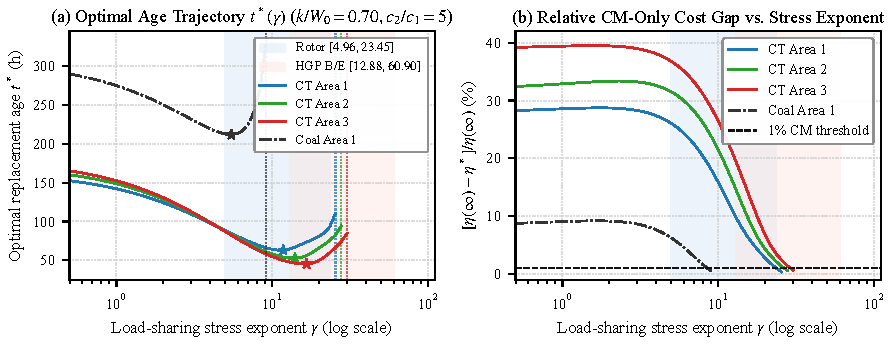
\includegraphics[width=14.5cm]{../figures/fig2_gamma_turning_point.pdf}
\caption{E3 turning-point sweep ($k/W_0 = 0.70, c_2/c_1 = 5$): (a) $t^*(\gamma)$ showing turning points and $<1\%$ corrective entry; (b) CM gap $[\eta(\infty)-\eta^*]/\eta(\infty)$ inside Rotor $[4.96, 23.45]$ and HGP B/E $[12.88, 60.90]$ envelopes.}
\label{fig:turning_point}
\end{figure}

\subsection{E4: four-dimensional consistency mapping for component-mix selection}
\label{sec:e4}

Because RTS-GMLC unit allocations ($m = 4$ \texttt{U20} units per CT area) reflect system-wide dispatch rather than station-level cost minimization, we map Policy~II mixes $m^*$ across $(r_{\mathrm{OM}}, \gamma, c_{pen}, k/W_0)$ ($3{,}750$ points plus $600$ Policy~I baselines) at fixed slot count $n$, treating $m = 4$ as a structural marker ($3 \le m^* \le 5$). Under fixed $n$, decreasing $m$ raises installed capacity $W_0(m)$ against fixed demand $k$, giving $m^* = 0$ an intrinsic reserve advantage alongside lower \texttt{U55} failure rates. Even under an equal-capacity control ($W_0 = 465\;\text{MW}$ in CT Area~1 at $k = 326\;\text{MW}, \gamma = 4.96, r_{\mathrm{OM}} = 1.96, c_{pen} = 15$), replacing $4\times\texttt{U55}$ with $11\times\texttt{U20}$ ($15\times\texttt{U20}+3\times\texttt{U55}$, $n=18$) raises $\eta_{II}^*$ from $0.111675$ to $0.168165$ because of higher aggregate outage frequency. Accordingly, all Policy~I cases ($600/600$) and symmetric Policy~II slices ($r_{\mathrm{OM}} = 1.00$, $750/750$) select $m^* = 0$, since \texttt{U20} carries a $2.15\times$ higher failure rate and smaller weight without an operating-cost discount.

Across the $3{,}000$ asymmetric Policy~II points ($r_{\mathrm{OM}} > 1$; Table~\ref{tab:case_e4_summary}, Figure~\ref{fig:e4_heatmap}), $30.17\%$ ($905/3{,}000$) yield interior mixes ($m^* \ge 1$) and $11.83\%$ ($355/3{,}000$) lie in $3 \le m^* \le 5$. Measuring percentage regret of a candidate mix $m_{\mathrm{ref}}$ as $[\eta_{II}(m_{\mathrm{ref}}, t^*(m_{\mathrm{ref}})) - \eta_{II}^*]/\eta_{II}^* \times 100\%$, evaluating $m = 4$ across all $905$ interior cells gives a median regret of $1.61\%$ (90th percentile $9.35\%$, maximum $27.73\%$; $553/905$ exceed $1\%$, compared with $0.21\%$ median and $6.84\%$ maximum within $3 \le m^* \le 5$). In contrast, forcing $m = 0$ across those $905$ cells incurs a median regret of $3.90\%$ (90th percentile $14.88\%$, maximum $31.18\%$; $708/905$ exceed $1\%$ and $197/905$ stay $\le 1\%$). Along the EIA slice $r_{\mathrm{OM}} = 1.96$ ($750$ points), $18.80\%$ ($141/750$) are interior and $7.73\%$ ($58/750$) lie in $3 \le m^* \le 5$ (per-area counts in Table~S7). Across those $141$ EIA interior cells, $m = 4$ yields median regret $1.16\%$ (90th percentile $5.75\%$, maximum $18.98\%$), dropping to $0.28\%$ median and $4.91\%$ maximum within $3 \le m^* \le 5$ ($0.45\%$--$0.50\%$ at $k/W_0 = 0.70, c_{pen} = 15, \gamma \in \{12.88, 23.45\}$). For comparison, forcing $m = 0$ on the EIA slice yields median regret $1.93\%$ (90th percentile $6.06\%$, maximum $12.17\%$; $99/141$ exceed $1\%$).

Cost-parameter checks on CT Area~1 ($k/W_0 = 0.70, \gamma = 12.88, r_{\mathrm{OM}} = 1.96, c_{pen} = 15$) show that $m^* = 3$ holds across $c_0 \in \{1.0, 2.0, 4.0\}$ ($m = 4$ regret $0.45\%$--$0.55\%$) and at $c_{ref,1} = 0.30$ ($0.33\%$), whereas reducing servicing to $c_{ref,1} = 0.05$ shifts the optimum to $m^* = 0$ ($3.46\%$). High outage penalties also restore the corner mix ($96.83\%$ at $c_{pen} = 100$). At $\gamma = 60.90$ with $r_{\mathrm{OM}} > 1$, $83.00\%$ ($249/300$; $86.40\%$ overall) select $m^* = 0$, leaving $17.00\%$ ($51/300$) interior (33 at $c_{pen}=10$, 16 at $c_{pen}=15$, and 2 at $c_{pen}=25$), with mixes reaching $m^* = 9$--$11$ at $r_{\mathrm{OM}} = 1.96$ and $m^* = 13$ in Area~3 at $k/W_0 = 0.50, c_{pen} \in \{10, 15\}, r_{\mathrm{OM}} \ge 2.50$.

\begin{table}[!t]
\centering
\scriptsize
\renewcommand{\arraystretch}{0.80}
\caption{Policy~II and Policy~I 4D parameter-box consistency summary pooled across CT Areas~1--3 (E4).}
\label{tab:case_e4_summary}
\begin{tabular*}{\textwidth}{@{\extracolsep{\fill}}lcccc@{}}
\toprule
Parameter Slice & Design Points & Corner ($m^* = 0$) & Band ($3 \le m^* \le 5$) & Any Interior ($m^* \ge 1$) \\
\midrule
Policy I (module replacement, no O\&M diff.) & 600   & 100.00\% (600)  & 0.00\% (0)     & 0.00\% (0) \\
Policy II full 4D box                        & 3,750 & 75.87\% (2,845) & 9.47\% (355)   & 24.13\% (905) \\
\midrule
Slice by unit O\&M ratio $r_{\mathrm{OM}} = 1.00$ & 750 & 100.00\% (750)  & 0.00\% (0)     & 0.00\% (0) \\
Slice by unit O\&M ratio $r_{\mathrm{OM}} = 1.50$ & 750 & 94.67\% (710)   & 1.07\% (8)     & 5.33\% (40) \\
EIA AEO 2026 slice $r_{\mathrm{OM}} = 1.96$       & 750 & 81.20\% (609)   & 7.73\% (58)    & 18.80\% (141) \\
Slice by unit O\&M ratio $r_{\mathrm{OM}} = 2.50$ & 750 & 58.93\% (442)   & 16.80\% (126)  & 41.07\% (308) \\
Slice by unit O\&M ratio $r_{\mathrm{OM}} = 3.00$ & 750 & 44.53\% (334)   & 21.73\% (163)  & 55.47\% (416) \\
\midrule
Asymmetric subset ($r_{\mathrm{OM}} > 1$), $c_{pen} = 10$  & 600 & 41.50\% (249) & 21.33\% (128) & 58.50\% (351) \\
Asymmetric subset ($r_{\mathrm{OM}} > 1$), $c_{pen} = 15$  & 600 & 55.17\% (331) & 17.33\% (104) & 44.83\% (269) \\
Asymmetric subset ($r_{\mathrm{OM}} > 1$), $c_{pen} = 100$ & 600 & 96.83\% (581) & 2.00\% (12)   & 3.17\% (19) \\
\bottomrule
\end{tabular*}
\end{table}

\begin{figure}[!t]
\centering
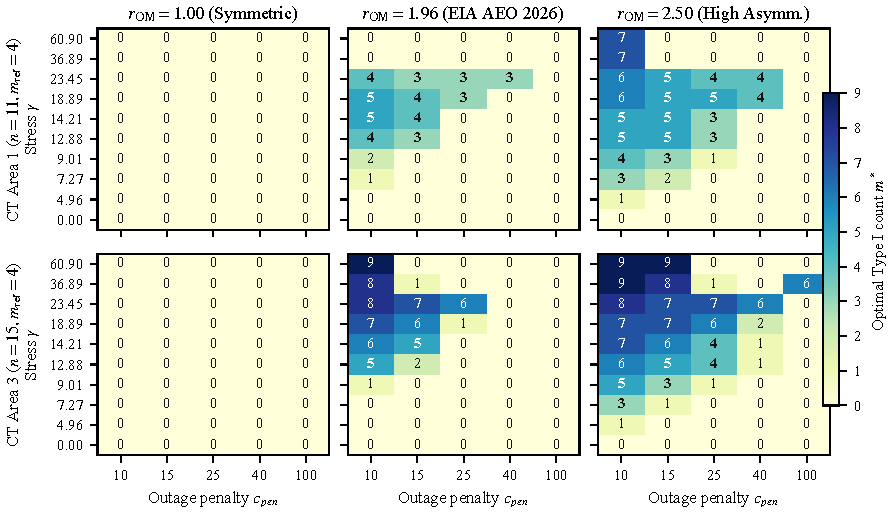
\includegraphics[width=14.0cm]{../figures/fig3_e4_consistency_heatmap.pdf}
\caption{Policy~II optimal $m^*$ across $\gamma$ and $c_{pen}$ at $k/W_0 = 0.70$ for CT Area~1 (top) and Area~3 (bottom) under $r_{\mathrm{OM}} \in \{1.00, 1.96, 2.50\}$ (bold: $3 \le m^* \le 5$).}
\label{fig:e4_heatmap}
\end{figure}

\subsection{E5: reverse-order coal array, swapped counterfactual, and CT comparison}
\label{sec:e5}

Table~\ref{tab:case_e5} contrasts Coal Area~1 ($\lambda_{2,0} > \lambda_{1,0}$), a fixed-geometry counterfactual Coal Area~1 (Swapped) ($\lambda_{1,0} \leftrightarrow \lambda_{2,0}$), and CT Areas~1--3 at $k/W_0 = 0.70, c_2/c_1 = 5$ (evaluating Coal across identical nominal $\gamma$ points solely as a controlled reverse-ordering benchmark rather than a steam-turbine OEM calibration). Because Coal Area~1 combines larger failure rates on \texttt{U155} ($\lambda_2/\lambda_1 = 2.04$, giving initial Type~II first-failure probability $P_1(\text{T-II}) = (n-m)\lambda_{2,0}/[m\lambda_{1,0}+(n-m)\lambda_{2,0}] = 60.49\%$) with large single-unit capacity share ($w_2/W_0 = 20.16\%$), its 1\%-CM threshold ($\gamma_{\mathrm{CM},1\%} = 9.12$, Table~S6) occurs $2.8\times$--$3.3\times$ earlier in $\gamma$ than in CT Areas~1--3 ($25.42$--$30.15$), while its turning point ($\gamma_{\mathrm{tp}} = 5.46$) occurs $2.2\times$--$3.0\times$ earlier than CT ($11.78$--$16.58$). Swapping failure rates alone on fixed Coal geometry lowers $P_1(\text{T-II})$ to $26.87\%$, restores finite PM at $\gamma = 12.88$ ($t^* = 212.62\;\text{h}$), shifts $\gamma_{\mathrm{tp}}$ from $5.46$ to $9.93$ ($70.7\%$ of the gap to CT Area~1 at $11.78$, $29.3\%$ residual geometry), and shifts $\gamma_{\mathrm{CM},1\%}$ from $9.12$ to $13.98$ ($29.8\%$ rate ordering, $70.2\%$ residual structural differences in $n$, weight ratio $w_2/w_1$, and capacity share $w_2/W_0$). In the reverse counterfactual (CT Area~1 geometry with Coal rates), $\gamma_{\mathrm{tp}} = 9.93$ and $\gamma_{\mathrm{CM},1\%} = 15.23$ assign $29.3\%$ and $62.5\%$ to rate ordering (Shapley averages $50.0\%$ and $46.2\%$, subject to $\approx \pm 4.5\%$ grid quantization from the $1.089$ ratio), confirming strong interaction between rate ordering and array geometry.

\begin{table}[htbp]
\centering
\scriptsize
\renewcommand{\arraystretch}{0.80}
\setlength{\tabcolsep}{2.2pt}
\caption{Reverse-order Coal Area~1, rate-swapped Coal counterfactual ($\lambda_1 \leftrightarrow \lambda_2$), and CT Areas~1--3 at $k/W_0 = 0.70, c_2/c_1 = 5$ (E5).}
\label{tab:case_e5}
\begin{tabular*}{\textwidth}{@{\extracolsep{\fill}}lccc|cc|cc|cc|cc@{}}
\toprule
 & & & & \multicolumn{2}{c|}{$\gamma = 0$} & \multicolumn{2}{c|}{Rotor $\rho=1.15$ ($4.96$)} & \multicolumn{2}{c|}{HGP $\rho=1.15$ ($12.88$)} & \multicolumn{2}{c}{Rotor $\rho=1.03$ ($23.45$)} \\
Array & Ordering & $P_1(\text{T-II})$ & $w_2/W_0$ & $\mathrm{MTTF}$ & $t^*$ & $\mathrm{MTTF}$ & $t^*$ & $\mathrm{MTTF}$ & $t^*$ & $\mathrm{MTTF}$ & $t^*$ \\
\midrule
Coal Area 1           & $\lambda_2 > \lambda_1$ & 60.49\% & 20.16\% & 465.25 & 307.29 & 304.31 & 212.68 & 225.80 & $\infty$ & 201.90 & $\infty$ \\
Coal Area 1 (Swapped) & $\lambda_1 > \lambda_2$ & 26.87\% & 20.16\% & 630.26 & 588.90 & 351.04 & 233.36 & 228.65 & 212.62   & 190.28 & $\infty$ \\
CT Area 1             & $\lambda_1 > \lambda_2$ & 44.83\% & 11.83\% & 345.32 & 164.17 & 182.89 & 88.58  & 108.25 & 64.46    & 81.97  & 93.58    \\
CT Area 2             & $\lambda_1 > \lambda_2$ & 51.10\% & 9.57\%  & 356.73 & 173.15 & 181.99 & 88.26  & 103.76 & 52.73    & 76.58  & 75.83    \\
CT Area 3             & $\lambda_1 > \lambda_2$ & 56.08\% & 8.03\%  & 360.65 & 179.46 & 180.44 & 87.22  & 100.13 & 47.67    & 72.17  & 60.16    \\
\bottomrule
\end{tabular*}
\end{table}

\subsection{E6: non-zero replacement duration sensitivity across duty factors}
\label{sec:e6}

To relax instantaneous replacement using reported RTS-GMLC repair durations ($d_{CM} \in \{31, 50\}\;\text{h}$ plus their unit-count-weighted array mean \texttt{WeightedAvg}, e.g., $37.91\;\text{h}$ for CT Area~1; $40\;\text{h}$ for Coal), we test preventive outage durations $d_{PM} \in \{d_{CM}/2, d_{CM}\}$ (spanning planned overhauls half as long as forced outages up to equal-duration renewals) alongside an explicit downtime opportunity-cost rate $c_d \ge 0$ per calendar hour of outage. Keeping $T_{sys}$ and $t^*$ in fired hours, duty factor $\delta \in \{1.00, 0.10\}$ defines the calendar-hour cost rate:
\begin{equation}
\eta_{\mathrm{cal}}(t; \delta, c_d) = \frac{c_1 + c_d d_{PM} + [c_2 - c_1 + c_d(d_{CM} - d_{PM})][1 - R_{sys}(t)]}{\delta^{-1}E[\min(T_{sys}, t)] + d_{PM} R_{sys}(t) + d_{CM}[1 - R_{sys}(t)]},
\label{eq:eta_cal_duty}
\end{equation}
spanning continuous ($\delta = 1.00$) and peaking ($\delta = 0.10$, EIA $\mathrm{CF} = 10\%$) duty across 3,360 E6 rows (Table~\ref{tab:case_e6} and Supplementary Table~S9). At $c_d = 0$, nonzero MTTRs lower $\eta_{\mathrm{cal}}^*$ relative to instantaneous replacement in all $2{,}628/2{,}628$ finite rows. At $k/W_0 = 0.70, c_2/c_1 = 5$ ($\delta = 1.00$), CT $t^*$ falls $3.71\%$--$20.99\%$ ($\gamma = 0$), $7.61\%$--$35.92\%$ ($\gamma = 4.96$), $24.60\%$--$72.47\%$ ($\gamma = 12.88$), and $61.24\%$--$95.37\%$ ($\gamma = 23.45$), while Coal contracts $13.08\%$--$30.30\%$ ($\gamma = 0$) and $21.54\%$--$45.36\%$ ($\gamma = 4.96$; $t^* = 71.06\;\text{h}$ at $\gamma = 12.88$ is a $c_d = 0$ dilution effect). Denominator inversion $c_1/d_{PM} < c_2/(\delta^{-1}\mathrm{MTTF} + d_{CM})$ affects $815$ of $2{,}628$ finite rows under $c_d = 0$: $775$ continuous rows (including $-95.37\%$, shrinking $t^*$ from $93.58$ to $4.34\;\text{h}$ rather than $0.50\;\text{h}$, and $\gamma = 60.90$ reaching $t_{lb} = 0.50\;\text{h}$) plus $40$ peaking rows at $c_2/c_1 = 20$ over $\gamma \in \{7.27, 12.88, 18.89, 23.45, 60.90\}$ (to $-96.76\%$). Across all $1{,}813$ non-inverted rows in the archive, contraction reaches $88.43\%$; within the $217$ non-inverted rows at $\delta = 1.00, c_2/c_1 = 5$, it reaches $82.99\%$ ($79.94\%$ across the $77$ rows at $k/W_0 = 0.70$, and $72.47\%$ for $\gamma \le 12.88$).

At peaking duty ($\delta = 0.10, c_2/c_1 = 5, c_d = 0$, $\delta d_{CM} = 3.1$--$5.0\;\text{h}$), CT $t^*$ shrinks by $0.39\%$--$2.63\%$ ($\gamma = 0$), $0.83\%$--$5.46\%$ ($\gamma = 4.96$), $3.17\%$--$19.50\%$ ($\gamma = 12.88$), and $9.78\%$--$38.91\%$ ($\gamma = 23.45$; lower bounds $0.39\%, 9.78\%$ in Table~S9). Conversely, corrective-rate downtime pricing $c_d = \delta c_2 / \mathrm{MTTF}$ gives $\eta_{\mathrm{cal}}(\infty; \delta, c_d) = c_d < c_1/d_{PM} + c_d = \eta_{\mathrm{cal}}(0^+; \delta, c_d)$ and removes inversions across all $2{,}628$ finite cases ($0/2{,}628$). At the benchmark $k/W_0 = 0.70, c_2/c_1 = 5$ slice across CT Areas~1--3 and $\gamma \in \{0, 4.96, 12.88, 23.45\}$, priced downtime slightly lengthens $t^*$ by $+0.92\%$--$+17.46\%$ under continuous duty and by $+0.12\%$--$+3.12\%$ under peaking duty (reaching its largest shift at $\gamma = 12.88$).

\begin{table}[htbp]
\centering
\scriptsize
\renewcommand{\arraystretch}{0.80}
\setlength{\tabcolsep}{1.8pt}
\caption{Selected E6 instantaneous versus non-zero MTTR sensitivity under unpenalized downtime ($c_d = 0$; $k/W_0 = 0.70, c_2/c_1 = 5$) for continuous ($\delta=1.00$) and peaking ($\delta=0.10$) duty, reporting fired $t^*$ (h) and calendar cost rate $\eta_{\mathrm{cal}}^*$.}
\label{tab:case_e6}
\begin{tabular*}{\textwidth}{@{\extracolsep{\fill}}llcc|cc|ccc|ccc@{}}
\toprule
 & & & & \multicolumn{2}{c|}{Instantaneous ($0,0$)} & \multicolumn{3}{c|}{$d_{PM} = d_{CM}/2$} & \multicolumn{3}{c}{$d_{PM} = d_{CM}$} \\
Array & $d_{CM}$ Basis & $\delta$ & $\gamma$ & $t^*$ & $\eta_{\mathrm{cal}}^*$ & $t^*$ & $\Delta t^*$ & $\eta_{\mathrm{cal}}^*$ & $t^*$ & $\Delta t^*$ & $\eta_{\mathrm{cal}}^*$ \\
\midrule
CT Area 1   & \texttt{U55} ($31$~h)     & 1.00 & 0.00  & 164.17 & 0.010453 & 154.49 & $-5.90\%$  & 0.009360 & 140.78 & $-14.25\%$ & 0.008628 \\
CT Area 1   & \texttt{U20} ($50$~h)     & 1.00 & 4.96  & 88.58  & 0.020203 & 72.84  & $-17.77\%$ & 0.014757 & 56.76  & $-35.92\%$ & 0.011766 \\
CT Area 1   & \texttt{U20} ($50$~h)     & 0.10 & 4.96  & 88.58  & 0.002020 & 86.70  & $-2.12\%$  & 0.001952 & 83.74  & $-5.46\%$  & 0.001904 \\
CT Area 1   & \texttt{U20} ($50$~h)     & 1.00 & 12.88 & 64.46  & 0.041601 & 32.45  & $-49.65\%$ & 0.024437 & 17.75  & $-72.47\%$ & 0.016660 \\
CT Area 1   & \texttt{U20} ($50$~h)     & 0.10 & 12.88 & 64.46  & 0.004160 & 59.27  & $-8.04\%$  & 0.003923 & 51.89  & $-19.50\%$ & 0.003793 \\
CT Area 1   & \texttt{U20} ($50$~h)     & 1.00 & 23.45 & 93.58  & 0.060382 & 20.54  & $-78.05\%$ & 0.032166 & 4.34   & $-95.37\%$ & 0.019156 \\
CT Area 1   & \texttt{U20} ($50$~h)     & 0.10 & 23.45 & 93.58  & 0.006038 & 77.65  & $-17.02\%$ & 0.005643 & 59.65  & $-36.26\%$ & 0.005522 \\
\midrule
CT Area 3   & \texttt{U20} ($50$~h)     & 1.00 & 4.96  & 87.22  & 0.017500 & 77.12  & $-11.58\%$ & 0.013027 & 65.73  & $-24.64\%$ & 0.010499 \\
CT Area 3   & \texttt{U20} ($50$~h)     & 1.00 & 23.45 & 60.16  & 0.066851 & 14.36  & $-76.14\%$ & 0.031321 & 6.43   & $-89.31\%$ & 0.018624 \\
CT Area 3   & \texttt{U20} ($50$~h)     & 0.10 & 23.45 & 60.16  & 0.006685 & 50.03  & $-16.84\%$ & 0.006161 & 36.75  & $-38.91\%$ & 0.005924 \\
\midrule
Coal Area 1 & \texttt{U76/155} ($40$~h) & 1.00 & 0.00  & 307.29 & 0.009857 & 267.10 & $-13.08\%$ & 0.008876 & 214.18 & $-30.30\%$ & 0.008370 \\
Coal Area 1 & \texttt{U76/155} ($40$~h) & 1.00 & 4.96  & 212.68 & 0.015397 & 166.88 & $-21.54\%$ & 0.013149 & 116.22 & $-45.36\%$ & 0.011952 \\
Coal Area 1 & \texttt{U76/155} ($40$~h) & 1.00 & 12.88 & $\infty$ & 0.022143 & $\infty$ & ---      & 0.018811 & 71.06  & ---        & 0.017355 \\
\bottomrule
\end{tabular*}
\end{table}

\subsection{Calibration limits and threats to validity}
Several boundaries frame interpretation. Because utility outage-load logs (e.g., North American Electric Reliability Corporation Generating Availability Data System, NERC GADS) are proprietary, $\gamma(\rho)$ over $\rho \in [1.03, 1.15]$ relies on (\ref{eq:proxy_hyp}) from OEM $+100^{\circ}\text{F}$ inspection multipliers \cite{ger3620} rather than direct hazard ratios or standardized MW deltas, excluding part-load regimes ($\mathrm{MF} < 1$). Unthrottled $k/W_0 = 0.50$ cascades extrapolate (\ref{eq:lam12}) near the discrete threshold bound, whereas nameplate capping limits stress to $1.15$.

The core model targets deferred-repair epochs with memoryless units, omitting Weibull wear-out, start fatigue, and continuous repair (though fast repair flattens hazards to CM in our baseline peaking check; higher cost ratios or stress can restore PM). E4 fixes $n$ and $k$ using uncalibrated servicing and setup ratios ($c_{ref,1} = 0.15, c_0 = 2.0$), where lower $c_{ref,1}$ collapses mixes to $m^* = 0$. Finally, E3 thresholds carry $\pm 4.5\%$ quantization, and $c_d = 0$ induces E6 denominator inversions below the CM asymptote.

\section{Conclusion and future work}
\label{sec:conclusion}

This study formulated an exact CTMC/PH framework for joint age replacement and component-mix optimization in heterogeneous weighted $k$-out-of-$n$:G systems under asymmetric TFR load sharing, proving variance--drift IFR conditions and extreme-stress boundary limits alongside a verified solver.

For engineering practice, the RTS-GMLC results yield four takeaways. First, within the calibrated $1.03$--$1.15$ band ($k/W_0 = 0.90$), neglecting load sharing adds at most $3.90\%$ ($c_2/c_1 = 5$) and $13.99\%$ ($c_2/c_1 = 20$), whereas deeper margins incur severe penalties under capped and unthrottled dispatch. Second, Type~II stress escalation dominates risk, fast online repair eliminates finite PM in the baseline peaking check, and turning-point capture tracks the overload band. Third, reverse-ordered coal clusters enter CM earlier than CT arrays via coupled rate ordering and geometry, while explicit downtime pricing removes calendar-rate inversions with modest peaking shifts. Fourth, Policy~II interior mixes require unit O\&M asymmetry when servicing costs matter. Future work will fit $\gamma_r$ from outage-load logs via maximum likelihood estimation, add wear-out and start fatigue, and test state-threshold policies \cite{hamdan2021,qi2024}.

\section*{Conflict of interest}
The author declares that there is no conflict of interest that could have influenced the conduct or presentation of this research.

\section*{Data availability statement}
Primary data come from the IEEE RTS-GMLC repository (\url{https://github.com/GridMod/RTS-GMLC}, commit \texttt{3ece0d37}); code, assertions, datasets, and Supplementary Material are provided for peer review in a blinded repository (public URL on the separate title page).

\begin{thebibliography}{60}\footnotesize
\setlength{\itemsep}{0pt}
\setlength{\parsep}{0pt}
\setlength{\parskip}{0pt}
\bibitem{rts1979} Probability Methods Subcommittee. IEEE Reliability Test System. IEEE Transactions on Power Apparatus and Systems 1979; PAS-98 (6): 2047-2054. doi: 10.1109/tpas.1979.319398
\bibitem{grigg1999} Grigg C, Wong P, Albrecht P, Allan R, Bhavaraju M et al. The IEEE Reliability Test System-1996. IEEE Transactions on Power Systems 1999; 14 (3): 1010-1020. doi: 10.1109/59.780914
\bibitem{billinton1996} Billinton R, Allan RN. Reliability Evaluation of Power Systems. 2nd ed. New York, NY, USA: Springer US, 1996. doi: 10.1007/978-1-4899-1860-4
\bibitem{billinton1994} Billinton R, Li W. Reliability Assessment of Electric Power Systems Using Monte Carlo Methods. New York, NY, USA: Springer US, 1994. doi: 10.1007/978-1-4899-1346-3
\bibitem{lisnianski2012} Lisnianski A, Elmakias D, Laredo D, Ben Haim H. A multi-state Markov model for a short-term reliability analysis of a power generating unit. Reliability Engineering \& System Safety 2012; 98 (1): 1-6. doi: 10.1016/j.ress.2011.10.008
\bibitem{ding2009} Ding Y, Lisnianski A, Wang P, Goel L, Chiang LP. Dynamic reliability assessment for bilateral contract electricity providers in restructured power systems. Electric Power Systems Research 2009; 79 (10): 1424-1430. doi: 10.1016/j.epsr.2009.04.014
\bibitem{wu1994} Wu JS, Chen RJ. An algorithm for computing the reliability of weighted-k-out-of-n systems. IEEE Transactions on Reliability 1994; 43 (2): 327-328. doi: 10.1109/24.295016
\bibitem{kuo2003} Kuo W, Zuo MJ. Optimal Reliability Modeling: Principles and Applications. Hoboken, NJ, USA: John Wiley \& Sons, 2003.
\bibitem{rushdi2018} Rushdi AM, Alturki AM. Novel representations for a coherent threshold reliability system: a tale of eight signal flow graphs. Turkish Journal of Electrical Engineering \& Computer Sciences 2018; 26: 257-269. doi: 10.3906/elk-1612-92
\bibitem{eryilmaz2014two} Eryilmaz S, Sarikaya K. Modeling and analysis of weighted-k-out-of-n:G system consisting of two different types of components. Proceedings of the Institution of Mechanical Engineers, Part O: Journal of Risk and Reliability 2014; 228 (3): 265-271. doi: 10.1177/1748006X13515647
\bibitem{eryilmaz2018} Eryilmaz S. The number of failed components in a k-out-of-n system consisting of multiple types of components. Reliability Engineering \& System Safety 2018; 175: 246-250. doi: 10.1016/j.ress.2018.03.027
\bibitem{qi2024} Qi F, Yang H, Wei L, Shu X. Preventive maintenance policy optimization for a weighted k-out-of-n:G system using the survival signature. Reliability Engineering \& System Safety 2024; 249: 110247. doi: 10.1016/j.ress.2024.110247
\bibitem{barlow1965} Barlow RE, Proschan F. Mathematical Theory of Reliability. New York, NY, USA: John Wiley \& Sons, 1965.
\bibitem{nakagawa1985} Nakagawa T. Continuous and discrete age-replacement policies. Journal of the Operational Research Society 1985; 36 (2): 147-154. doi: 10.1057/jors.1985.28
\bibitem{nakagawa2005} Nakagawa T. Maintenance Theory of Reliability. London, UK: Springer-Verlag, 2005. doi: 10.1007/1-84628-221-7
\bibitem{wang2006} Wang H, Pham H. Reliability and Optimal Maintenance. London, UK: Springer-Verlag, 2006. doi: 10.1007/b138077
\bibitem{hamdan2021} Hamdan K, Tavangar M, Asadi M. Optimal preventive maintenance for repairable weighted k-out-of-n systems. Reliability Engineering \& System Safety 2021; 205: 107267. doi: 10.1016/j.ress.2020.107267
\bibitem{fotuhi2014} Fotuhi-Firuzabad M, Aminifar F, Shahzadeh A. Reliability-based maintenance scheduling of generating units in restructured power systems. Turkish Journal of Electrical Engineering \& Computer Sciences 2014; 22: 1147-1158. doi: 10.3906/elk-1208-79
\bibitem{almuhaini2017} Almuhaini M, Al-Sakkaf A. Markovian model for reliability assessment of microgrids considering load transfer restriction. Turkish Journal of Electrical Engineering \& Computer Sciences 2017; 25: 4657-4672. doi: 10.3906/elk-1609-137
\bibitem{barrows2020} Barrows C, Preston E, Staid A, Stephen G, Watson JP et al. The IEEE Reliability Test System: a proposed 2019 update. IEEE Transactions on Power Systems 2020; 35 (1): 119-127. doi: 10.1109/tpwrs.2019.2925557
\bibitem{ger3620} Beagle D, Moran B, McDufford M, Merine M. Heavy-duty gas turbine operating and maintenance considerations. Technical Report GER-3620 Rev P. Atlanta, GA, USA: GE Vernova, 2021.
\bibitem{eia2026} U.S. Energy Information Administration. Assumptions to the Annual Energy Outlook 2026: Electricity Market Module. Washington, DC, USA: U.S. Department of Energy, 2026.
\bibitem{li2008} Li W, Zuo MJ. Reliability evaluation of multi-state weighted k-out-of-n systems. Reliability Engineering \& System Safety 2008; 93 (1): 160-167. doi: 10.1016/j.ress.2006.11.009
\bibitem{eryilmaz2015mttf} Eryilmaz S. Mean time to failure of weighted k-out-of-n: G systems. Communications in Statistics - Simulation and Computation 2015; 44 (10): 2705-2713. doi: 10.1080/03610918.2013.844836
\bibitem{eryilmaz2015} Eryilmaz S. Capacity loss and residual capacity in weighted k-out-of-n:G systems. Reliability Engineering \& System Safety 2015; 136: 140-144. doi: 10.1016/j.ress.2014.12.008
\bibitem{eryilmaz2021} Eryilmaz S, Ucum KA. The lost capacity by the weighted k-out-of-n system upon system failure. Reliability Engineering \& System Safety 2021; 216: 107914. doi: 10.1016/j.ress.2021.107914
\bibitem{hamdan2024} Hamdan K, Asadi M, Tavangar M. On reliability assessment of weighted k-out-of-n systems with multiple types of components. Quality Technology \& Quantitative Management 2024; 21 (5): 656-673. doi: 10.1080/16843703.2023.2238339
\bibitem{qi2026} Qi F, Yang H, Liu Y, Chen X, Kong J. Condition-based maintenance for a multi-state weighted k-out-of-n:G system considering stochastic dependency. International Journal of Production Research 2026; 64 (9): 3690-3706. doi: 10.1080/00207543.2025.2592804
\bibitem{golmohamadi2014} Golmohamadi H, Ramezani M, Falaghi H. Competitive unit maintenance scheduling in a deregulated environment based on preventing market power. Turkish Journal of Electrical Engineering \& Computer Sciences 2014; 22: 529-545. doi: 10.3906/elk-1207-69
\bibitem{heidari2016} Heidari A, Alizadeh Pahlavani MR. An advanced optimization technique for considering reliability issues and unit commitment problems simultaneously. Turkish Journal of Electrical Engineering \& Computer Sciences 2016; 24: 1061-1074. doi: 10.3906/elk-1310-218
\bibitem{hashemi2013} Hashemi-Dezaki H, Hosseinian SH, Askarian-Abyaneh H, Agah SMM. Optimized operation and maintenance costs to improve system reliability by decreasing the failure rate of distribution lines. Turkish Journal of Electrical Engineering \& Computer Sciences 2013; 21: 2191-2204. doi: 10.3906/elk-1203-34
\bibitem{kumari2026} Kumari R, Naick BK. Distribution system reliability evaluation considering protection coordination using Petri nets. Turkish Journal of Electrical Engineering \& Computer Sciences 2026; 34 (1): 49-66. doi: 10.55730/1300-0632.4162
\bibitem{daniels1945} Daniels HE. The statistical theory of the strength of bundles of threads. I. Proceedings of the Royal Society of London. Series A. Mathematical and Physical Sciences 1945; 183 (995): 405-435. doi: 10.1098/rspa.1945.0011
\bibitem{liu1998} Liu H. Reliability of a load-sharing k-out-of-n:G system: non-iid components with arbitrary distributions. IEEE Transactions on Reliability 1998; 47 (3): 279-284. doi: 10.1109/24.740502
\bibitem{amari2008} Amari SV, Bergman R. Reliability analysis of k-out-of-n load-sharing systems. In: 2008 Annual Reliability and Maintainability Symposium; 2008. pp. 440-445. doi: 10.1109/rams.2008.4925836
\bibitem{taghipour2015} Taghipour S, Kassaei ML. Periodic inspection optimization of a k-out-of-n load-sharing system. IEEE Transactions on Reliability 2015; 64 (3): 1116-1127. doi: 10.1109/tr.2015.2421819
\bibitem{liu2016} Liu B, Xie M, Kuo W. Reliability modeling and preventive maintenance of load-sharing systems with degrading components. IIE Transactions 2016; 48 (8): 699-709. doi: 10.1080/0740817X.2015.1125041
\bibitem{che2020} Che H, Zeng S, Guo J. A reliability model for load-sharing k-out-of-n systems subject to soft and hard failures with dependent workload and shock effects. Eksploatacja i Niezawodnosc - Maintenance and Reliability 2020; 22 (2): 253-264. doi: 10.17531/ein.2020.2.8
\bibitem{huang2023} Huang X, Xu L, Huang Y, Fang Y. Reliability analysis for k-out-of-N:F load sharing systems operating in a shock environment. IEEE Access 2023; 11: 18227-18233. doi: 10.1109/access.2023.3247449
\bibitem{jamali2022} Arabzadeh Jamali M, Pham H. Opportunistic maintenance model for load sharing k-out-of-n systems with perfect PM and minimal repairs. Quality Engineering 2022; 34 (2): 205-214. doi: 10.1080/08982112.2022.2033774
\bibitem{hao2024} Hao Y, Zhu X. Redundancy design and preventive maintenance for a load-sharing multiasset system considering uncertain environmental conditions. IEEE Transactions on Industrial Informatics 2024; 20 (7): 9308-9319. doi: 10.1109/tii.2024.3383492
\bibitem{ghnimi2025} Ghnimi S, Mannai N. Optimal redundancy allocation for a k-out-of-n:G load-sharing system with random mission duration. Annals of Operations Research 2025. doi: 10.1007/s10479-025-06957-2
\bibitem{mannai2026} Mannai N, Jarray M. Optimal design of k-out-of-n:G system under load redistribution and stochastic mission duration. Reliability Engineering \& System Safety 2026; 269: 112029. doi: 10.1016/j.ress.2025.112029
\bibitem{zhao2025} Zhao S, Wei Y, Cheng Y, Li Y. A state-specific joint size, maintenance, and inventory policy for a k-out-of-n load-sharing system subject to self-announcing failures. Reliability Engineering \& System Safety 2025; 257: 110855. doi: 10.1016/j.ress.2025.110855
\bibitem{sharifi2023} Sharifi M, Taghipour S. Inspection interval optimization of a weighted-K-out-of-N system with identical multi-state load-sharing components. Reliability Engineering \& System Safety 2023; 238: 109412. doi: 10.1016/j.ress.2023.109412
\end{thebibliography}

\end{document}
